%%%%%%%%%%%%%%%%%%%%%%%%%%%%%%%%%%%%%%%%%
% Beamer Presentation
% LaTeX Template
% Version 1.0 (10/11/12)
%
% This template has been downloaded from:
% http://www.LaTeXTemplates.com
%
% License:
% CC BY-NC-SA 3.0 (http://creativecommons.org/licenses/by-nc-sa/3.0/)
%
%%%%%%%%%%%%%%%%%%%%%%%%%%%%%%%%%%%%%%%%%

%----------------------------------------------------------------------------------------
%	PACKAGES AND THEMES
%----------------------------------------------------------------------------------------

\documentclass{beamer}
\usepackage{xcolor}
\usepackage{graphicx}
\usepackage{listings}
\usepackage{multicol}

\definecolor{applegreen}{rgb}{0.55, 0.71, 0.0}
\definecolor{blue(ncs)}{rgb}{0.0, 0.45, 0.60}
\definecolor{burgundy}{rgb}{0.5, 0.0, 0.13}


\mode<presentation> {

\usetheme{CambridgeUS}

\usecolortheme{wolverine}

\definecolor{gold}{HTML}{D4A017}
\definecolor{darkgold}{HTML}{B7950B}

\setbeamercolor{palette primary}{bg=gold,fg=white}
\setbeamercolor{palette secondary}{bg=darkgold,fg=white}
\setbeamercolor{palette tertiary}{bg=black,fg=white}
\setbeamercolor{palette quaternary}{bg=gold,fg=white}

\setbeamercolor{frametitle}{bg=darkgold,fg=white}

\setbeamercolor{section number projected}{bg=black,fg=gold}
\setbeamercolor{item}{fg=black,bg=gold}

\setbeamertemplate{page number in head/foot}[framenumber]
}

\usepackage{graphicx} % Allows including images
\usepackage{booktabs} % Allows the use of \toprule, \midrule and \bottomrule in tables

%----------------------------------------------------------------------------------------
%	TITLE PAGE
%----------------------------------------------------------------------------------------

\title[libCEED Finite Element Library]{Optimizing Performance for Portable Generic Finite Element Interfaces} % The short title appears at the bottom of every slide, the full title is only on the title page

\author{Jeremy L Thompson} % Your name
\institute[CU Boulder] % Your institution as it will appear on the bottom of every slide, may be shorthand to save space
{University of Colorado Boulder \\ % Your institution for the title page
\medskip
\textit{jeremy.thompson@colorado.edu} % Your email address
}
\date{February 27, 2019} % Date, can be changed to a custom date

\begin{document}

\begin{frame}
\titlepage % Print the title page as the first slide
\end{frame}

%------------------------------------------------

\begin{frame}
\begin{center}
\frametitle{libCEED Team}

{\flushleft

Developers: \hspace{2mm} Jed Brown\textsuperscript{1}, Jeremy Thompson\textsuperscript{1} \\
\hspace{23mm} Valeria Barra\textsuperscript{1}, Tzanio Kolev\textsuperscript{2}, Jean-Sylvain Camier\textsuperscript{2},\\
\hspace{23mm} Veselin Dobrev\textsuperscript{2}, Yohann Doudouit\textsuperscript{2}, Tim Warburton\textsuperscript{3},\\
\hspace{23mm} David Medina\textsuperscript{4}, \& Thilina Rathnayake\textsuperscript{5}\\

~\\

Grant: \hspace{11mm} Exascale Computing Project (17-SC-20-SC)\\

~\\

~\\

\small{1: University of Colorado, Boulder\\
2: Lawrence Livermore National Laboratory\\
3: Virginia Polytechnic Institute and State University\\
4: OCCA\\
5: University of Illinois, Urbana-Champaign\\}}

\end{center}
\end{frame}

\begin{frame}
\begin{center}
\frametitle{Overview}

A global sparse matrix is no longer a good representation of\\high-order linear operators\\

~\\

libCEED is an extensible library that provides a portable\\algebraic interface and optimized implementations\\

~\\

We have optimized implementations using\\SIMD intrinsics and LIBXSMM

~\\

We have results comparing performance on\\CEED benchmark problems

\end{center}
\end{frame}
 
%------------------------------------------------

\begin{frame}
\frametitle{Overview} % Table of contents slide, comment this block out to remove it
\tableofcontents % Throughout your presentation, if you choose to use \section{} and \subsection{} commands, these will automatically be printed on this slide as an overview of your presentation
\end{frame}

%----------------------------------------------------------------------------------------
%	PRESENTATION SLIDES
%----------------------------------------------------------------------------------------

%------------------------------------------------
\section{Introduction}
%------------------------------------------------

\begin{frame}
\begin{center}
\frametitle{Center for Efficient Exascale Discretizations}

\begin{flushleft}
DoE exascale co-design center
\end{flushleft}

\begin{itemize}

\item Design discretization algorithms for exascale hardware that deliver significant performance gain over low order methods

\item Collaborate with hardware vendors and software projects for exascale hardware and software stack

\item Provide efficient and user-friendly unstructured PDE discretization component for exascale software ecosystem

\end{itemize}

\end{center}
\end{frame}

%------------------------------------------------
\section{libCEED}
%------------------------------------------------

\begin{frame}
\begin{center}
\frametitle{Design Philosophy}

\begin{multicols}{2}

\begin{flushright}
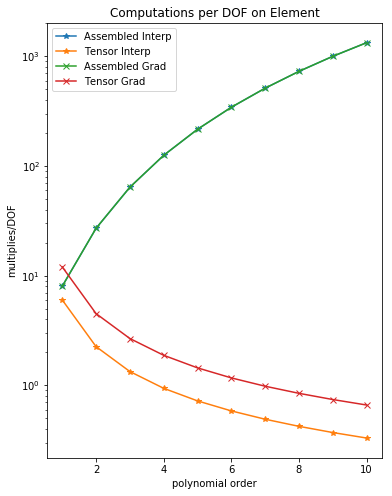
\includegraphics[height=5cm]{libCEEDAssembledVsTensorApply}
\end{flushright}

\begin{flushleft}
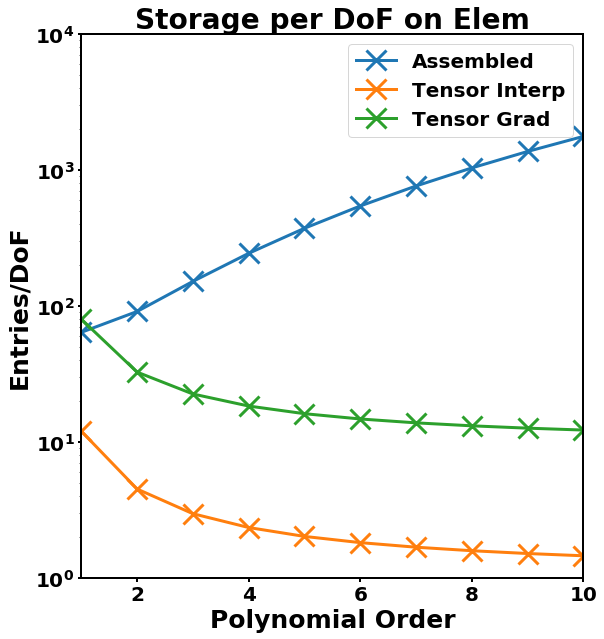
\includegraphics[height=5cm]{libCEEDAssembledVsTensorStorage}
\end{flushleft}

\end{multicols}

Using an assembled matrix inhibits performance optimizations\\
for hexahedral elements

\end{center}
\end{frame}

%------------------------------------------------

\begin{frame}
\begin{center}
\frametitle{Matrix Free}

libCEED design approach:

\begin{itemize}

\item Avoid global matrix assembly

\item Map each element to reference element

\item Geometry data computed on the fly or precomputed

\item Easy to parallelize across hetrogeneous nodes

\end{itemize}

\end{center}
\end{frame}

%------------------------------------------------

\begin{frame}
\begin{center}
\frametitle{libCEED}

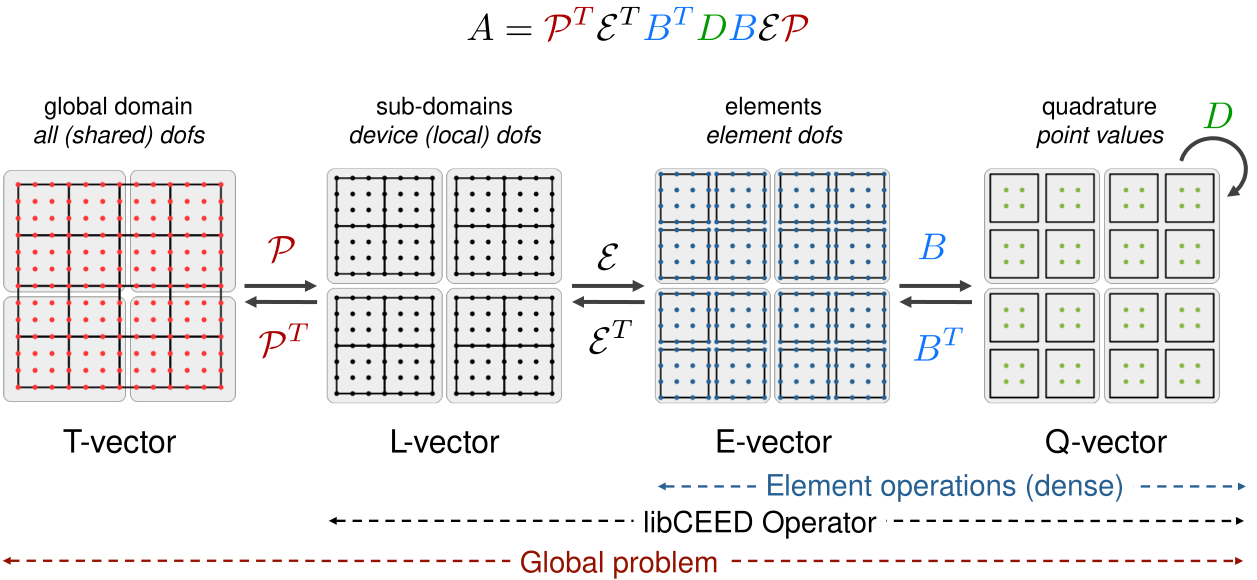
\includegraphics[height=4.5cm]{libCEEDAPI}

\small{

\hspace{1.8cm}${\color{burgundy}A}_L = G^T {\color{blue(ncs)}B^T} {\color{applegreen}D} {\color{blue(ncs)}B} G$

\begin{itemize}

\item $G$ - CeedElemRestriction, local gather/scatter

\item {\color{blue(ncs)}$B$} - CeedBasis, provides basis operations such as interp and grad

\item {\color{applegreen}$D$} - CeedQFunction, representation of PDE at quadrature points

\item ${\color{burgundy}A}_L$ - CeedOperator, aggregation of Ceed objects for local action of operator

\end{itemize}

}

\end{center}
\end{frame}

%------------------------------------------------

\begin{frame}
\begin{center}
\frametitle{libCEED}

libCEED provides multiple backend implementations

\begin{itemize}

\item CPU

\begin{itemize}

\item Pure C

\item Advanced Vector Instructions

\item LIBXSMM

\end{itemize}

\item GPU

\begin{itemize}

\item Pure CUDA

\item OCCA

\item MAGMA

\end{itemize}

\end{itemize}

\end{center}
\end{frame}

%------------------------------------------------
\section{Optimization}
%------------------------------------------------

\begin{frame}
\begin{center}
\frametitle{SIMD Intrinsics}

\begin{itemize}

\item Provides parallelism on multicore CPUs\\

~\\

\item Better compiled code without writing assembly\\

~\\

\item We target architectures with AVX support

\end{itemize}

\end{center}
\end{frame}

%------------------------------------------------

\begin{frame}
\begin{center}
\frametitle{LIBXSMM}

\begin{itemize}

\item Small matrix multiplication kernels\\

~\\

\item $\left( M N K \right)^{1 / 3} \leq 128$\\

~\\

\item Targets Intel architectures\\

~\\

\item JIT code specialization for compiler independent performance

\end{itemize}

\end{center}
\end{frame}

%------------------------------------------------

\begin{frame}
\begin{center}
\frametitle{Vectorization}

\begin{itemize}

\item Internal vectorization

\begin{itemize}

\item Serial element processing

\item Matrix dimensions may not fit vector length evenly

\end{itemize}

\item External vectorization

\begin{itemize}

\item Blocked element processing

\item Fewer edge cases

\item Gather/scatter needs to interlace elements

\end{itemize}

\end{itemize}

\end{center}
\end{frame}

%------------------------------------------------
\section{Benchmarks}
%------------------------------------------------

\begin{frame}
\begin{center}
\frametitle{Benchmark Problems}

\begin{multicols}{2}

\begin{flushleft}
Benchmark Problem 1:
\end{flushleft}

\begin{itemize}

\item $B u = f$

\item $L^2$ projection problem

\end{itemize}

\begin{flushleft}
Benchmark Problem 3:
\end{flushleft}

\begin{itemize}

\item $A u = f$

\item Poisson problem

\end{itemize}

\end{multicols}

\begin{flushleft}

~\\

3D scalar problem\\

$p \in \left\{ 1 ... 16 \right\}$, $q = p + 2$\\

$p$ - polynomial degree, $q$ - number of quadrature nodes\\

Unpreconditioned CG, maximum of 20 iterations

~\\

Compare performance across multiple implementations

\end{flushleft}

\end{center}
\end{frame}

%------------------------------------------------

\begin{frame}
\begin{center}
\frametitle{Machine Specs}

\begin{itemize}

\item CU Summit\\

~\\

\item Intel Xeon E5-2680 v3, 24 cores/node\\

~\\

\item Omni-Path HF1 interconnect\\

~\\

\item Using 4 full nodes, no special location

\end{itemize}

\end{center}
\end{frame}

%------------------------------------------------

\begin{frame}
\begin{center}
\frametitle{Decoding Results}

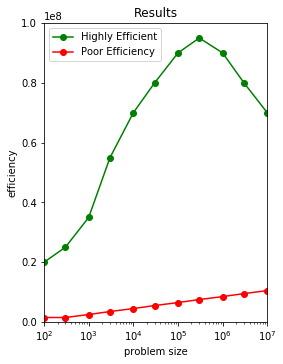
\includegraphics[width=5cm]{libCEEDBenchKey}

\vspace{-0.1cm}

\begin{itemize}

\footnotesize{

\item Horizontal axis - Problem size, points per compute node

\item Vertical axis - Efficiency, [DOFs x CG Iterations] / [Compute Nodes x
Seconds]

}

\end{itemize}

\end{center}
\end{frame}

%------------------------------------------------

\begin{frame}
\begin{center}
\frametitle{BP 1 Baseline}

\begin{multicols}{2}

\begin{flushleft}
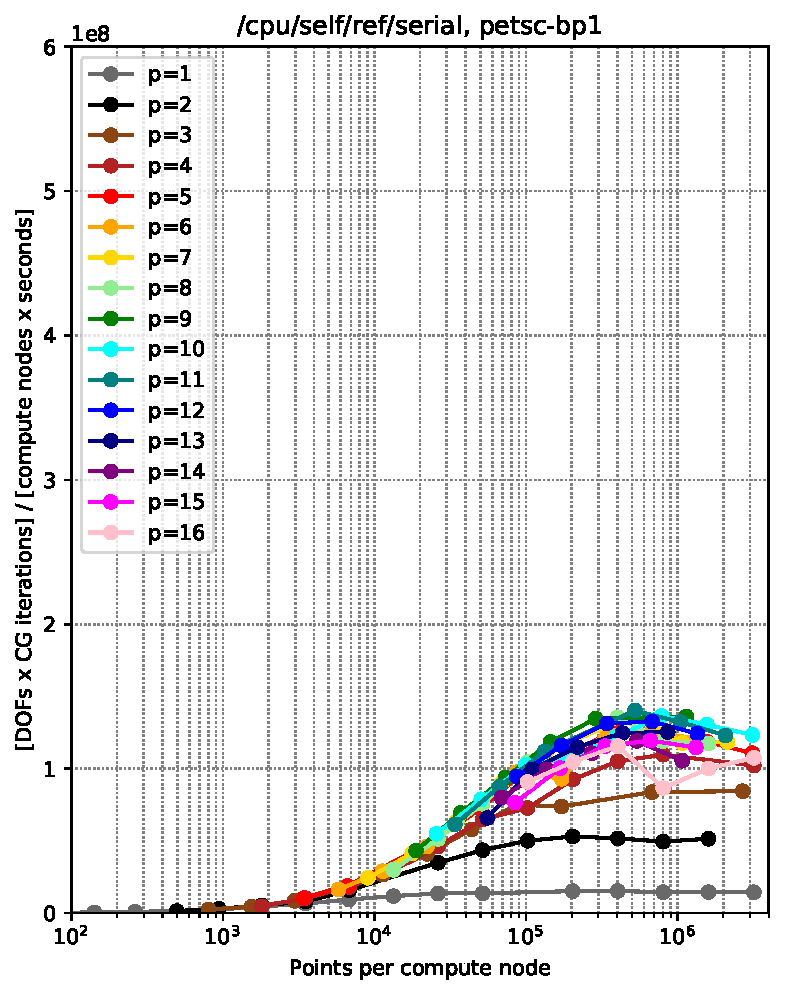
\includegraphics[width=5cm]{plot_libCEED_petsc-bp1_cpuselfrefserial_N004_pn24.pdf}
\end{flushleft}

\begin{flushright}
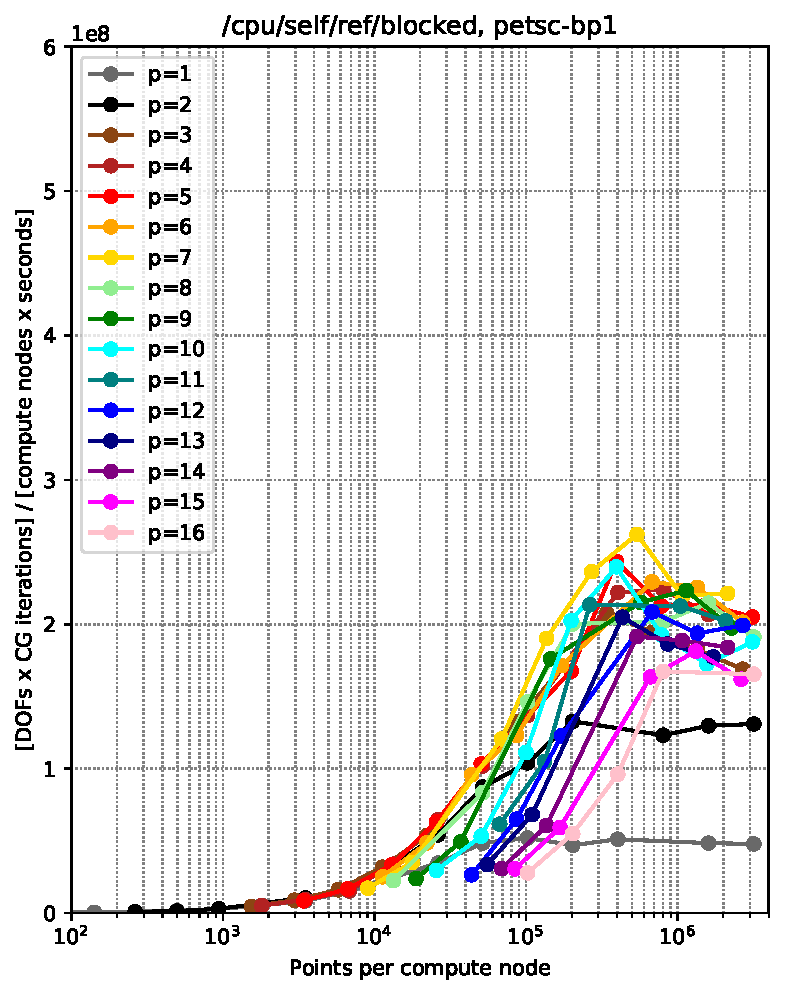
\includegraphics[width=5cm]{plot_libCEED_petsc-bp1_cpuselfrefblocked_N004_pn24.pdf}
\end{flushright}

\end{multicols}

\vspace{-0.15cm}

\begin{itemize}

\item Better blocked performance

\end{itemize}

\end{center}
\end{frame}

%------------------------------------------------

\begin{frame}
\begin{center}
\frametitle{BP 1 AVX Results}

\begin{multicols}{2}

\begin{flushleft}
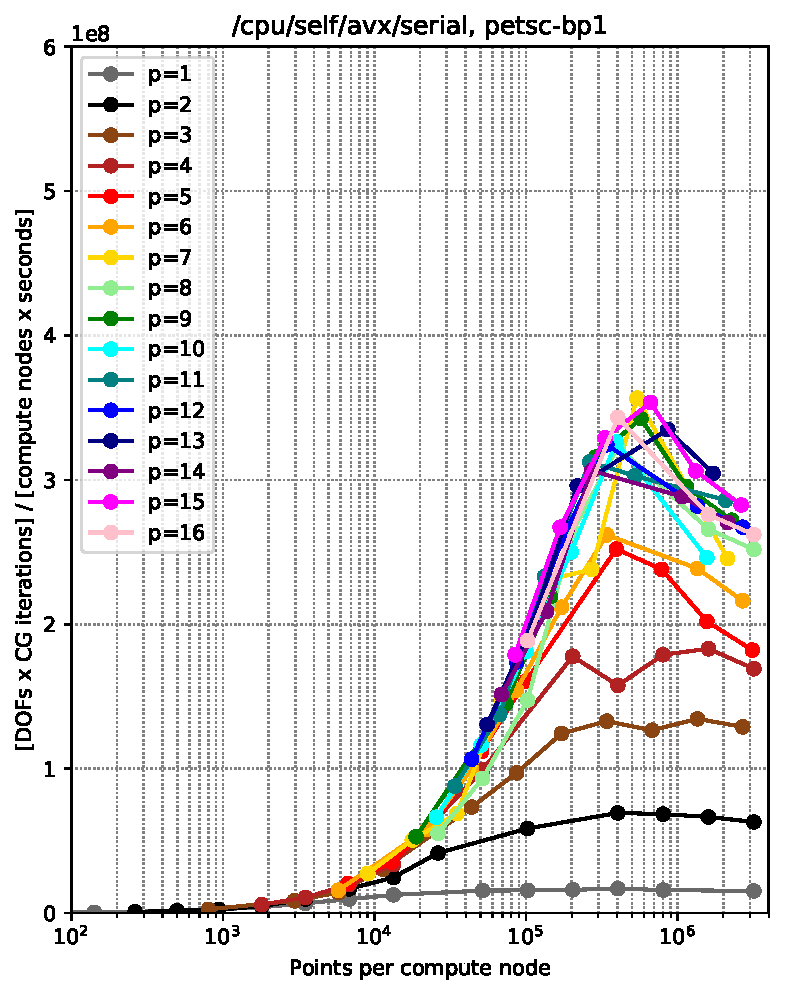
\includegraphics[width=5cm]{plot_libCEED_petsc-bp1_cpuselfavxserial_N004_pn24.pdf}
\end{flushleft}

\begin{flushright}
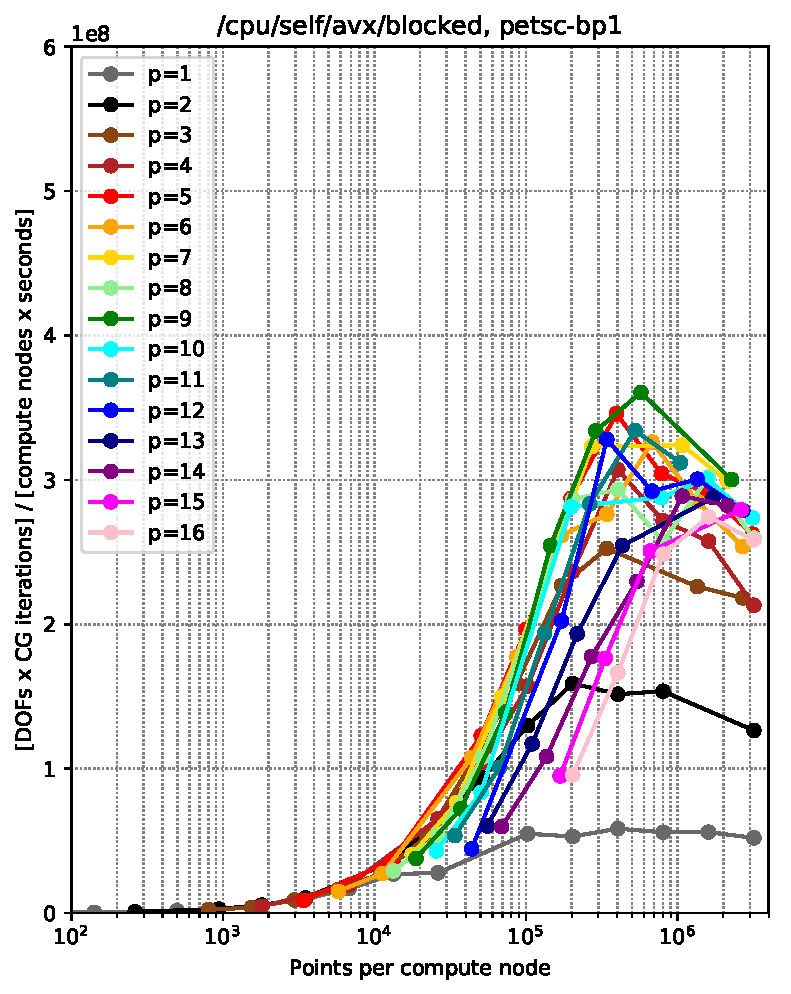
\includegraphics[width=5cm]{plot_libCEED_petsc-bp1_cpuselfavxblocked_N004_pn24.pdf}
\end{flushright}

\end{multicols}

\vspace{-0.15cm}

\begin{itemize}

\item $p \leq 7$ better blocked performance, $p > 7$ better serial performance

\end{itemize}

\end{center}
\end{frame}

%------------------------------------------------

\begin{frame}
\begin{center}
\frametitle{BP 1 LIBXSMM Results}

\begin{multicols}{2}

\begin{flushleft}
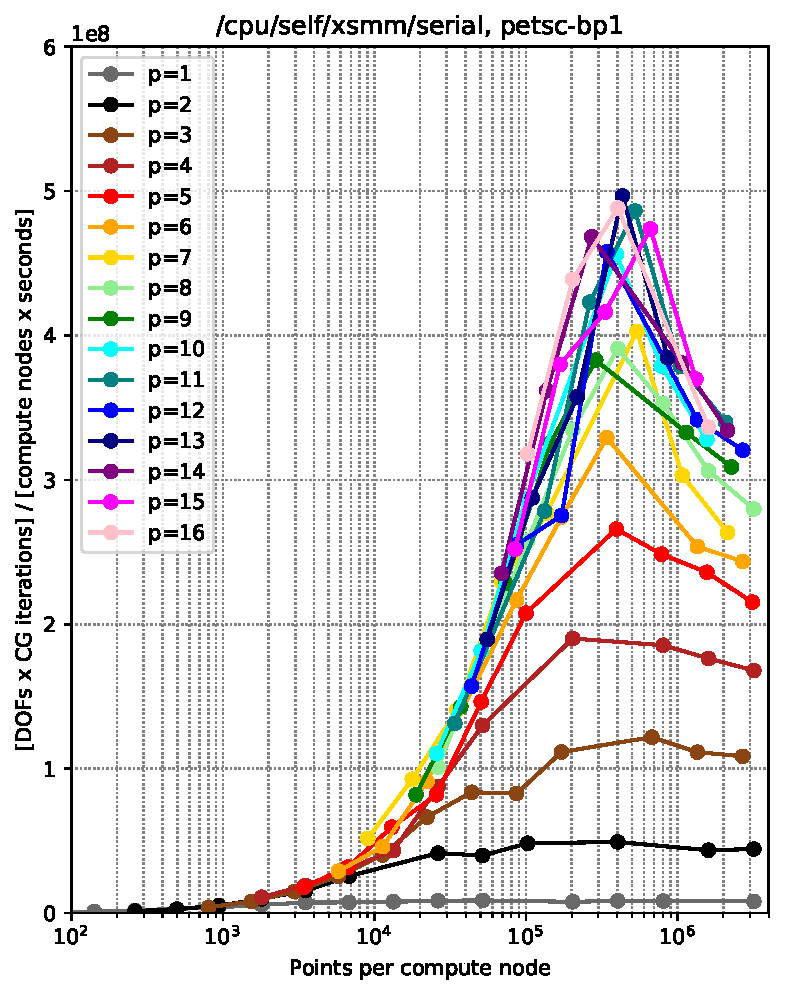
\includegraphics[width=5cm]{plot_libCEED_petsc-bp1_cpuselfxsmmserial_N004_pn24.pdf}
\end{flushleft}

\begin{flushright}
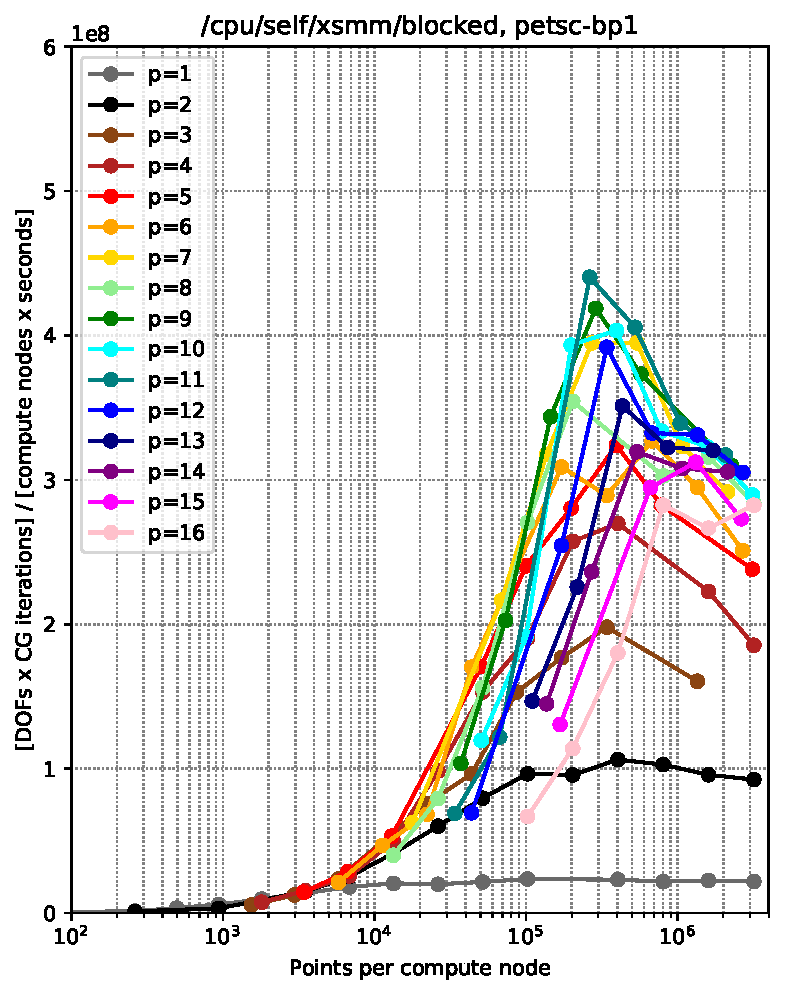
\includegraphics[width=5cm]{plot_libCEED_petsc-bp1_cpuselfxsmmblocked_N004_pn24.pdf}
\end{flushright}

\end{multicols}

\vspace{-0.5cm}

\begin{itemize}

\item $p \leq 7$ better blocked performance, $p > 7$ better serial performance

\item LIBXSMM handles internal vectorization much better

\end{itemize}

\end{center}
\end{frame}

%------------------------------------------------

\begin{frame}
\begin{center}
\frametitle{BP 3 Baseline}

\begin{multicols}{2}

\begin{flushleft}
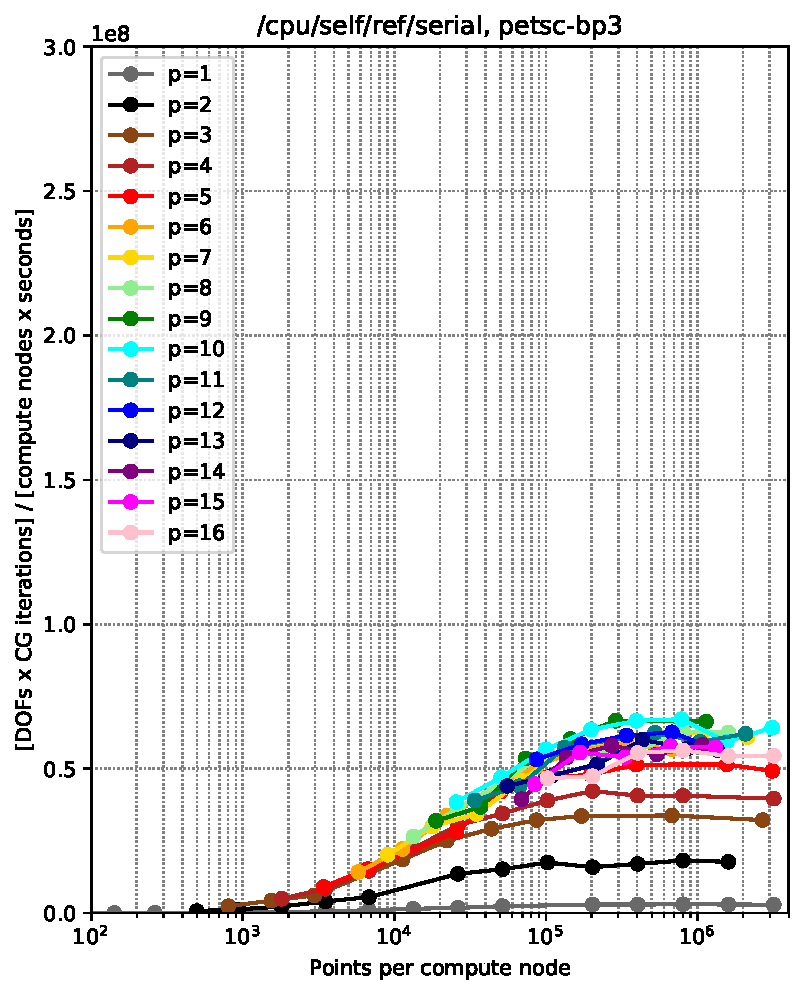
\includegraphics[width=5cm]{plot_libCEED_petsc-bp3_cpuselfrefserial_N004_pn24.pdf}
\end{flushleft}

\begin{flushright}
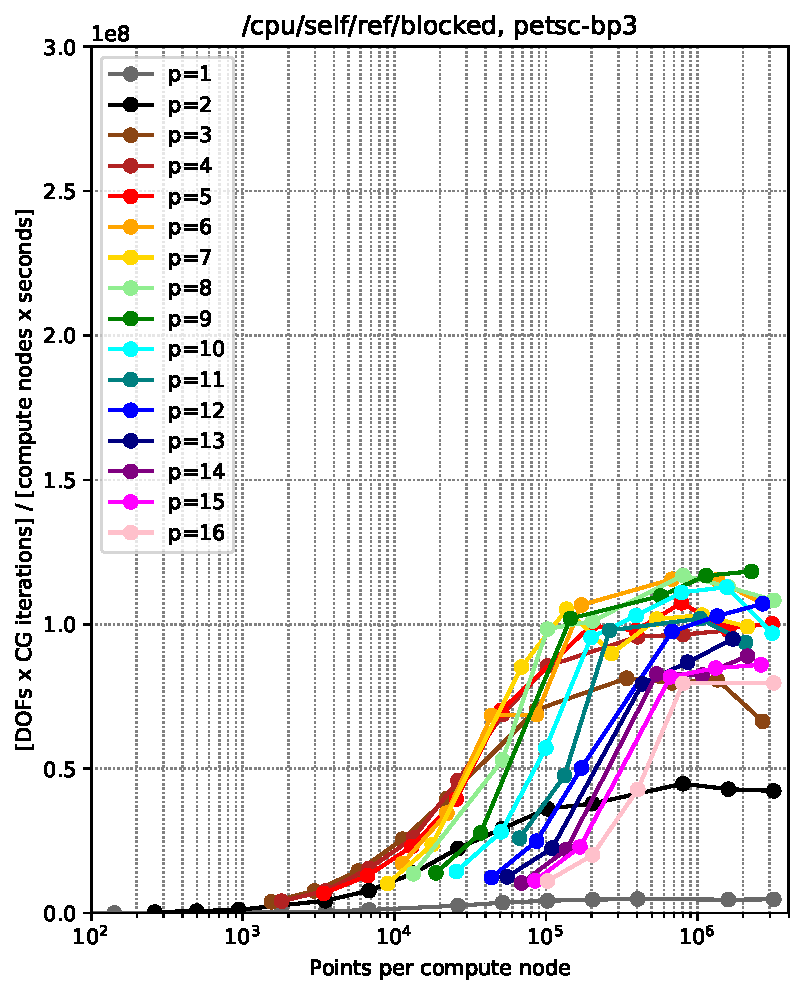
\includegraphics[width=5cm]{plot_libCEED_petsc-bp3_cpuselfrefblocked_N004_pn24.pdf}
\end{flushright}

\end{multicols}

\vspace{-0.15cm}

\begin{itemize}

\item Better blocked performance

\end{itemize}

\end{center}
\end{frame}

%------------------------------------------------

\begin{frame}
\begin{center}
\frametitle{BP 3 AVX Results}

\begin{multicols}{2}

\begin{flushleft}
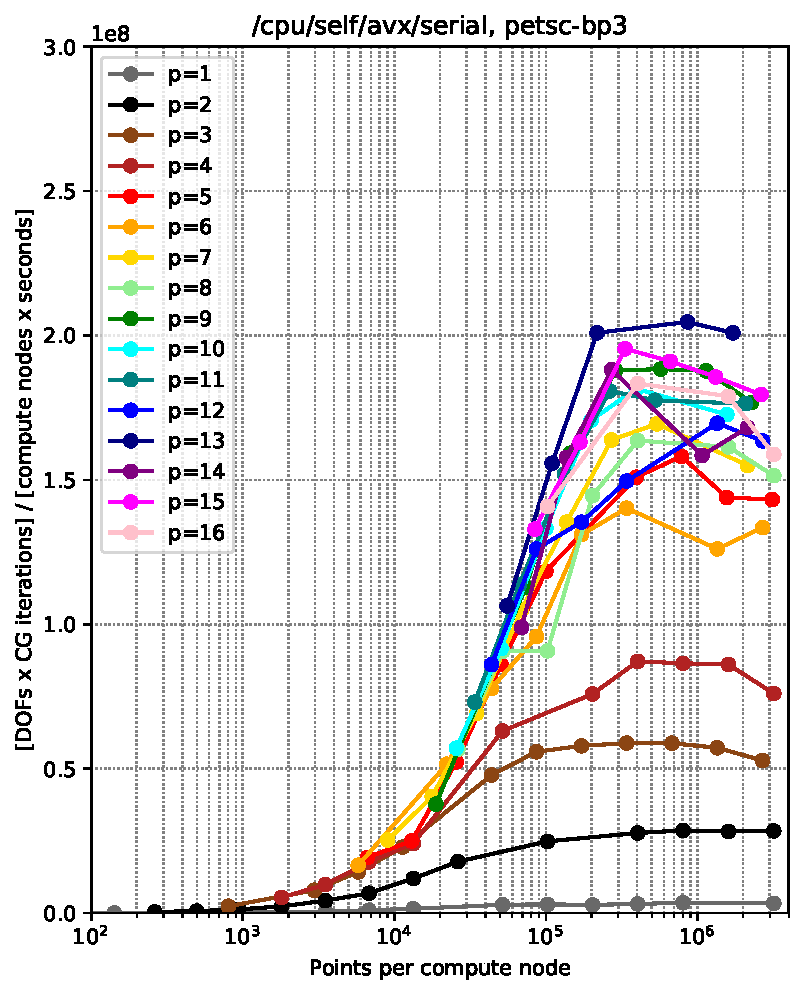
\includegraphics[width=5cm]{plot_libCEED_petsc-bp3_cpuselfavxserial_N004_pn24.pdf}
\end{flushleft}

\begin{flushright}
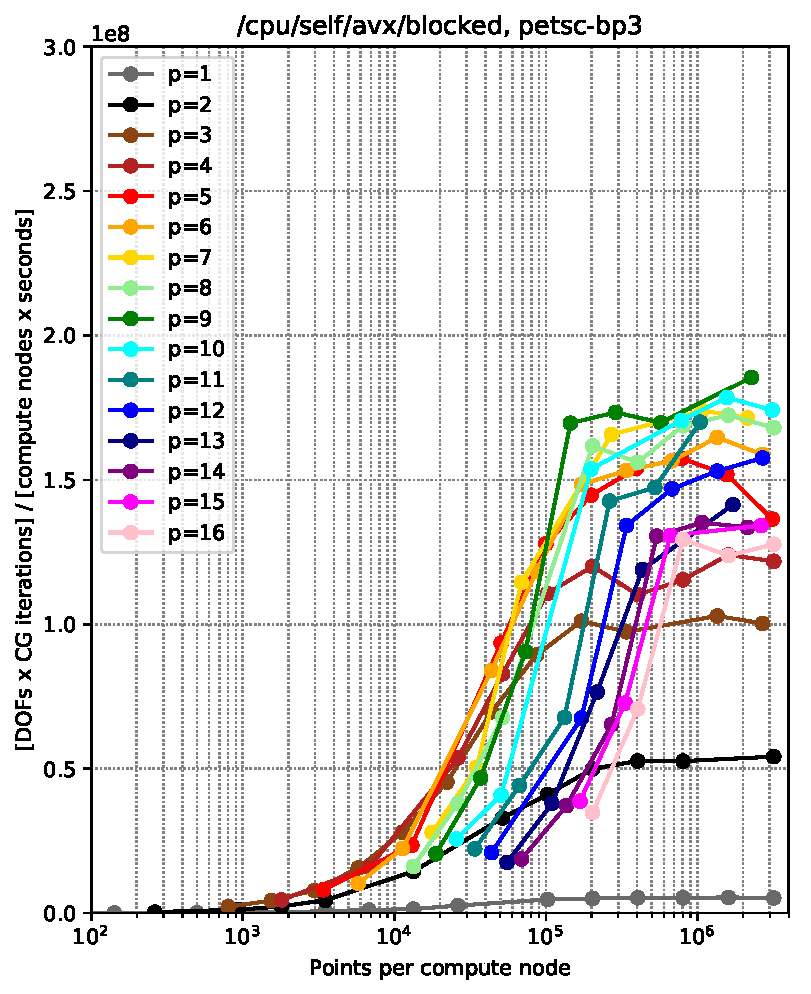
\includegraphics[width=5cm]{plot_libCEED_petsc-bp3_cpuselfavxblocked_N004_pn24.pdf}
\end{flushright}

\end{multicols}

\vspace{-0.15cm}

\begin{itemize}

\item $p \leq 7$ better blocked performance, $p > 7$ better serial performance

\end{itemize}

\end{center}
\end{frame}

%------------------------------------------------

\begin{frame}
\begin{center}
\frametitle{BP 3 LIBXSMM Results}

\begin{multicols}{2}

\begin{flushleft}
\includegraphics[width=5cm]{plot_libCEED_petsc-bp3_cpuselfxsmmserial_N004_pn24.pdf}
\end{flushleft}

\begin{flushright}
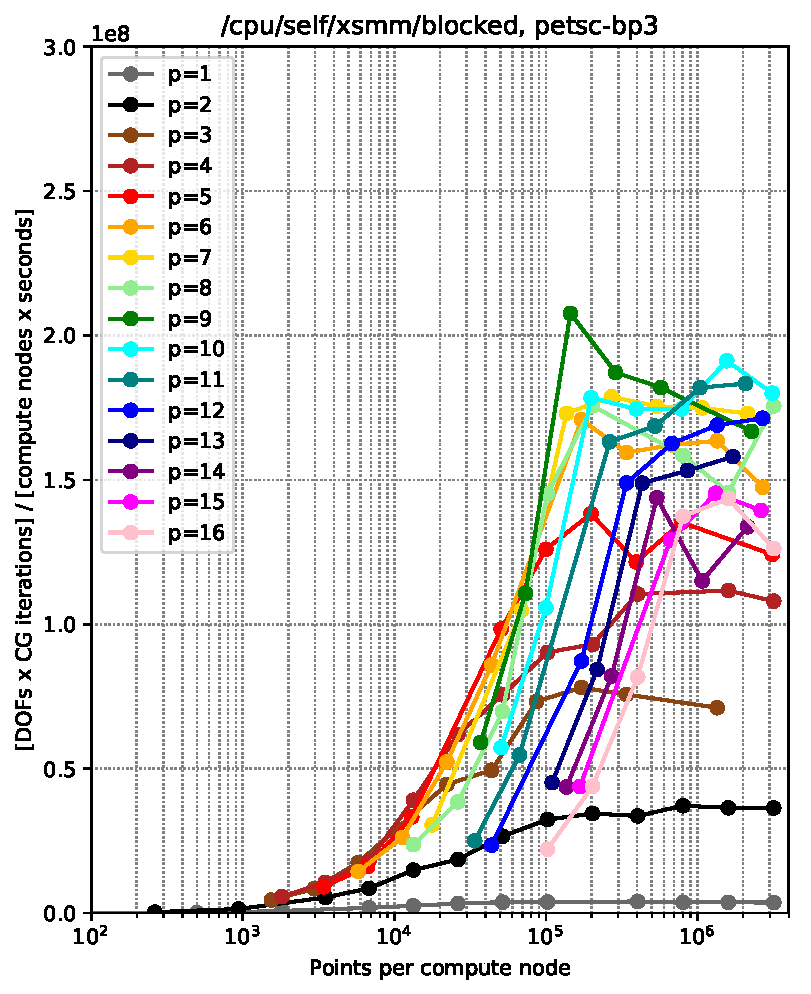
\includegraphics[width=5cm]{plot_libCEED_petsc-bp3_cpuselfxsmmblocked_N004_pn24.pdf}
\end{flushright}

\end{multicols}

\vspace{-0.5cm}

\begin{itemize}

\item $p \leq 7$ better blocked performance, $p > 7$ better serial performance

\item LIBXSMM handles internal vectorization much better

\end{itemize}

\end{center}
\end{frame}

%------------------------------------------------
\section{Future Work}
%------------------------------------------------

\begin{frame}
\begin{center}
\frametitle{Future Work}

\begin{itemize}

\item Further performance tuning\\

~\\

\item Improved non-conforming and mixed mesh support\\

~\\

\item Algorithmic differentiation of quadrature functions\\

~\\

\item We invite contributors and friendly users

\end{itemize}

\end{center}
\end{frame}

%------------------------------------------------
\section{Questions}
%------------------------------------------------

\begin{frame}
\begin{center}
\frametitle{Questions?}

{\flushleft

Advisor: \hspace{8mm} Jed Brown\textsuperscript{1}\\

~\\

Collaborators: Valeria Barra\textsuperscript{1}, Tzanio Kolev\textsuperscript{2}, Jean-Sylvain Camier\textsuperscript{2},\\
\hspace{23mm} Veselin Dobrev\textsuperscript{2}, Yohann Doudouit\textsuperscript{2}, Tim Warburton\textsuperscript{3},\\
\hspace{23mm} David Medina\textsuperscript{4}, \& Thilina Rathnayake\textsuperscript{5}\\

~\\

Grant: \hspace{11mm} Exascale Computing Project (17-SC-20-SC)\\

~\\

~\\

\small{1: University of Colorado, Boulder\\
2: Lawrence Livermore National Laboratory\\
3: Virginia Polytechnic Institute and State University\\
4: OCCA\\
5: University of Illinois, Urbana-Champaign\\}}

\end{center}
\end{frame}

%------------------------------------------------

\begin{frame}[noframenumbering]
\titlepage % Print the title page
\end{frame}

%------------------------------------------------

%----------------------------------------------------------------------------------------

\end{document}

